\newchapstyle
\chapter{Current phase relations of graphene Josephson junctions in microwave circuits}
\label{chap:gJJ-CPR}

\blfootnote{
	\color{title}
	This chapter is based on previously unpublished data of the devices presented in Chapter~\ref{chap:gJJ}.
	%
	Data and code to reproduce the calculations and figures presented here can be found on Zenodo~\cite{schmidtDataCodeCurrent2020}.
}

\begin{abstract}
	We perform extensive analysis of graphene Josephson junctions embedded in microwave circuits.
	%
	By comparing a diffusive junction at \SI{15}{\milli\kelvin} with a ballistic one at \SI{15}{\milli\kelvin} and \SI{1}{\kelvin}, we are able to reconstruct the current-phase relation.
\end{abstract}

%% Start the actual chapter on a new page.
\newpage

\section{Introduction}

Josephson junctions (JJs) are widely used in microwave (MW) applications, such as quantum limited amplification and sensing, where they are being exploited as nonlinear inductors.
%
For the use of JJs in superconducting quantum information circuits, the junction nonlinearity has a major effect on the circuit requirements and capabilities~\cite{kringhojAnharmonicitySuperconductingQubit2018}.
%
However, the exact Josephson inductance can significantly differ between junctions:
%
While JJs are generally non-linear elements, the specific non-linearity depends on the current-phase relation (CPR) which in turn is determined by the underlying physics inside the junction.

The current-phase relation is a fundamental property of the JJ, relating the supercurrent $I_J$ flowing across a weak link between two superconducting banks with the phase difference $\delta$ between the two superconductors.
%
It results from the first derivative of the Josephson energy potential with respect to phase, $I_J(\delta) = (2e/\hbar) \partial V(\delta)/\partial \delta$.
%
For the ideal case of a JJ formed by a thin insulating tunnel barrier between two superconducting electrodes (SIS), the Josephson potential is given by $V(\delta)=1-E_J\cos\delta$ and the CPR has pure sinusoidal character as given by the first Josephson relation, $I_J(\delta) = I_c\sin\delta$~\cite{josephsonPossibleNewEffects1962,josephsonSupercurrentsBarriers1965}.

However, in JJs formed by normal conductors between superconductors (SNS) such as graphene Josephson junctions (gJJs), transport across the JJ is governed by Andreev bound states, each with ground state energy
\begin{align}
V_i(\delta)=1-\Delta_0\sqrt{1-\tau_i\sin^2(\delta/2)}
\label{eq:ABSenergy}
\end{align}
%
with transmission probability $\tau$ and superconducting gap $\Delta_0$~\cite{beenakkerUniversalLimitCriticalcurrent1991,titovJosephsonEffectBallistic2006b}.
%
Assuming equal $\tau$ for all channels, i.e. $\tau=\sum\tau_i/N$, the corresponding CPR is given by
\begin{align}
I_J(\delta) = \frac{\pi\Delta_0}{2 e R_n} \frac{\sin\delta}{\sqrt{1 - \tau \sin^2(\delta / 2)}},
\label{eq:CPR-ball}
\end{align}
%
with the Boltzmann constant $k_B$ and normal state resistance $R_n= R_q/N = h/(Ne^2)\approx \SI{25.812}{\kilo\ohm} / N$~\cite{golubovCurrentphaseRelationJosephson2004a,leeUltimatelyShortBallistic2015}.
%
Here, $R_q$ denotes the quantum Hall resistance and $N$ the number of conducting channels.
%
Depending on $\tau$, the CPR can exhibit significant forward skew compared to the case of a purely sinusoidal CPR in SIS JJs.
%
While the CPR of gJJs has been studied in the DC regime~\cite{englishObservationNonsinusoidalCurrentphase2016,nandaCurrentPhaseRelationBallistic2017}, and gJJs have been successfully incorporated in MW circuits~\cite{schmidtBallisticGrapheneSuperconducting2018,krollMagneticFieldCompatible2018,wangCoherentControlHybrid2019}, the influence of the potentially skewed CPR has not been studied in the latter.

Here, we analyze the effect of a nonlinear CPR on the microwave performance of gJJ embedded in microwave circuits.
%
Measuring two devices in different states, we compare the influence of scattering transport and temperature on the JJ nonlinearity.
%
Our circuit design allows in-situ, and even simultaneous, DC and MW measurements, providing us with various measurement types to compare.
%
The results show the usefulness of combining DC and MW in the same circuits for fundamental research on Josephson junction physics, which distinguishes it from pure MW CPR measurements~\cite{rifkinCurrentphaseRelationPhasedependent1976}.

\section{Circuit characterization}

Our circuit consists of a DC-bias microwave cavity formed by a coplanar waveguide (CPW) which is shunted by a large capacitor at the input, and shorted to ground on the far end by a gJJ that can be tuned with a gate voltage ($V_g$), cf. Fig.~\ref{fig:figure1}(a) and Refs.~\cite{schmidtBallisticGrapheneSuperconducting2018,schmidtCurrentDetectionUsing2020,bosmanBroadbandArchitectureGalvanically2015c}.
%
The superconducting base layer and shunt capacitor metal layers consist of DC-sputtered molybdenum-rhenium on a sapphire substrate, while the shunt capacitor dielectric layer is PECVD-\ce{SiN_x}.
%
The gate voltage lead is fed through a second shunt capacitor of the same geometry as the one at the input in order to suppress MW radiation leaking in through or out of the gate line.
%
The MW wiring of both samples was fabricated on a single \SI{2}{inch} sapphire wafer, after which the wafer was diced into \SI{10x10}{\milli\meter} pieces onto which the individual gJJ were placed.
%
The gJJ consist of boron nitride encapsulated single layer graphene with side-contacts of DC-sputtered niobium titanium nitride (NbTiN), fabricated via the etch-fill technique~\cite{wangOneDimensionalElectricalContact2013b,schmidtBallisticGrapheneSuperconducting2018}
%
The gJJ are designed to be \SI{5}{\micro\meter} wide and separate the NbTiN leads by a length of \SI{500}{\nano\meter}.
%
Gate tunability is achieved by placing a third NbTiN lead extending over the entire gJJ, separated by a bilayer of HSQ.
%
The circuit is wirebonded into a PCB that is mounted on the millikelvin plate of a dilution refrigerator and connected to the outside world via a bias-T, allowing both DC and MW characterization in the same setup.
%
To suppress thermal excitations, the MW inout line is heavily attenuated and all DC lines were equipped with $\pi$-filters in the room temperature battery powered electronics, as well as copper powder and two-stage RC filters thermally anchored to the millikelvin stage.

We measured two separate devices with nominally identical microwave circuits and junction designs:
%
One of the devices exhibited signatures of ballistic transport in form of Fabry-Pérot-like oscillations, which we will refer to as the \textit{ballistic device}, which is the device presented in the main text of Ref.~\cite{schmidtBallisticGrapheneSuperconducting2018}.
%
The other one, in lack of such features, will be called \textit{diffusive device}, and corresponds to the reference sample of the same reference, cf. Supplementary Material Sec.~\ref{sec:ballistic} and Fig.~\ref{fig:SMFig-ballistic} for details on the ballistic features.
%
With a normal state resistance of both devices ranging between \SIrange{35}{350}{\ohm}, depending on gate voltage, we estimate around 74 to 740 conducting channels.
%
This justifies the use of a single averaged transparency parameter $\tau$ in Eq.~\ref{eq:ABSenergy}.

We extract the DC circuit parameters by applying a bias current to the JJ, using the CPW as a long capacitive lead and measuring the voltage drop across the gJJ.
%
When exceeding a critical current, the JJ switches from the zero-voltage to the resistive state.
%
We record this switching current $I_c$ for varying gate voltages, as depicted in Fig.~\ref{fig:figure1}(b,c) for the two devices at a base temperature of \SI{15}{\milli\kelvin} in the case of the diffusive, and both base temperature and \SI{1}{\kelvin} for the ballistic device.
%
In line with a minimum conductivity even at the CNP~\cite{katsnelsonZitterbewegungChiralityMinimal2006, zieglerRobustTransportProperties2006, tworzydloSubPoissonianShotNoise2006,titovJosephsonEffectBallistic2006b}, there remains a finite supercurrent in both samples, that cannot be pinched off completely.
%
The DC switching current of the diffusive device ranges from a few hundred \si{\nano\ampere} to \SI{5.5}{\micro\ampere}, similar to the ballistic device at \SI{1}{\kelvin}.
%
At base temperature, the maximum $I_c$ of the ballistic device reaches up to \SI{7.5}{\micro\ampere}.
%
Both samples exhibit significantly larger switching current for $V_g>V_{\rm CNP}$ (n-doping) compared to $V_g<V_{\rm CNP}$ (p-doping), where $V_{\rm CNP}$ denotes the gate voltage at the charge neutrality point (CNP) of the gJJ.
%
We attribute this to a reduced contact transparency in the p-doped regime~\cite{schmidtBallisticGrapheneSuperconducting2018}.
%
We measure $V_{\rm CNP}^{\rm diff}=\SI{1.55}{\volt}$ and $V_{\rm CNP}^{\rm ball}=\SI{-1.39}{\volt}$ for the diffusive and ballistic sample, respectively.
%
Discrepancies are presumably due to differences in residual doping during fabrication.

\begin{figure}[t]
	\centering
	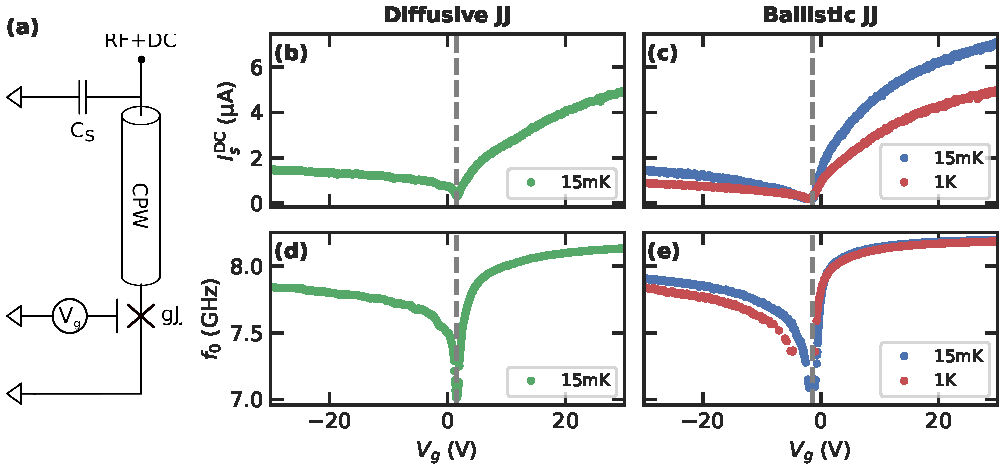
\includegraphics[width=\linewidth]{chapter-gJJ-CPR/figs/Figure1}
	\caption{
		\textbf{Simultaneous MW and DC measurements of ballistic and diffusive graphene Josesphson junctions.}
		%
		\textbf{(a)} Measurement schematic.
		%
		The gJJ shorts a coplanar waveguide transmission line to ground, which forms a gate-tunable $\lambda/2$-resonator.
		%
		$V_g$ is fed through an additional shunt capacitor (not shown).
		\textbf{(b,c)} Switching current for the diffusive \textbf{(b)} and ballistic Josephson junction \textbf{(c)}, at base-temperature of \SI{15}{\milli\kelvin} (blue) and at \SI{1}{\kelvin} (red).
		%
		\textbf{(d,e)} Resonance frequencies versus gate voltage for the diffusive \textbf{(d)} and ballistic \textbf{(e)} device.
		%
		The gate-tunable Josephson inductance changes the boundary condition of the $\lambda/2$-resonator, thus changing the resonance frequency of the circuit.
		%
		Dashed grey lines indicate the charge neutrality point of each device, marked by the minimum critical current.
	}
	\label{fig:figure1}
\end{figure}

For high frequency signals, i.e. a few \si{\giga\hertz}, the gJJ behaves as a nonlinear inductor, with Josephson inductance
%
\begin{align}
L_J = \frac{\hbar}{2e}\left(\diff{I_J}{\delta}\right)^{-1},
\label{eq:LJgeneral}
\end{align}
%
which can be derived from the second Josephson relation, $\partial\delta/\partial t=2e V/\hbar$.
%
Depending on the impedance of the gJJ at the circuit resonance frequency, $Z_J=i\omega_0 L_J$, the fundamental mode hosted by the gJJ-terminated CPW varies between a $\lambda/2$ wave for $Z_J\rightarrow0$ and $\lambda/4$ for $Z_J\rightarrow\infty$.

The resonance frequency of a $\lambda/2$-resonator shorted to ground by a Josephson inductance can be approximated by
\begin{align}
f_0\left(I_b,I_c\right) = f_{\lambda/2} \frac{L_r+L_J\left(I_b, I_c\right)}{L_r +  2L_J\left(I_b, I_c\right)}
\label{eq:Pogorzalek}
\end{align}
%
with $L_r$ the bare CPW inductance and $f_{\lambda/2}$ the resonance frequency of the CPW without the JJ, see Supplementary Material Sec.~\ref{sec:calibration}.
%
$I_b$ is the bias current flowing through CPW and the JJ, $I_c$ the critical current of the JJ.
%
We can immediately see that for small $L_J$, $f_0\rightarrow f_{\lambda/2}$, while for $L_J\gg L_r$, $f_0 \rightarrow f_{\lambda/2}/2$.

The circuit response is measured by recording the reflection coefficient $S_{11}$ of the cavity using a vector network analyzer, which excites the device through a series of attenuators and a directional coupler, and measures the reflected signal, amplified by low noise cryogenic and room temperature HEMTs. 
%
We fit the response using an analytical model to extract resonance frequency $f_0$ and internal ($\kappa_i$) and external loss rates ($\kappa_e$), cf. Supplementary Material Sec.~\ref{sec:extraction}.
%
We observe gate-tunable resonance frequency $f_0$ between \SIrange{7.0}{8.2}{\giga\hertz}, comparable for both devices, cf. Fig.~\ref{fig:figure1}(d,e).
%
Due to the inverse nature of junction current and inductance, the large changes in $I_c$ for $V_g>V_{\rm CNP}$ only lead to minor changes in $f_0$ when comparing the hot and cold ballistic device.
%
On the other hand, even small changes in the significantly smaller $I_c$ for $V_g<V_{\rm CNP}$ significantly reduce $f_0$ in this regime.

\section{Deviations between Josephson inductance from DC and MW measurements}

\begin{figure}[t]
	\centering
	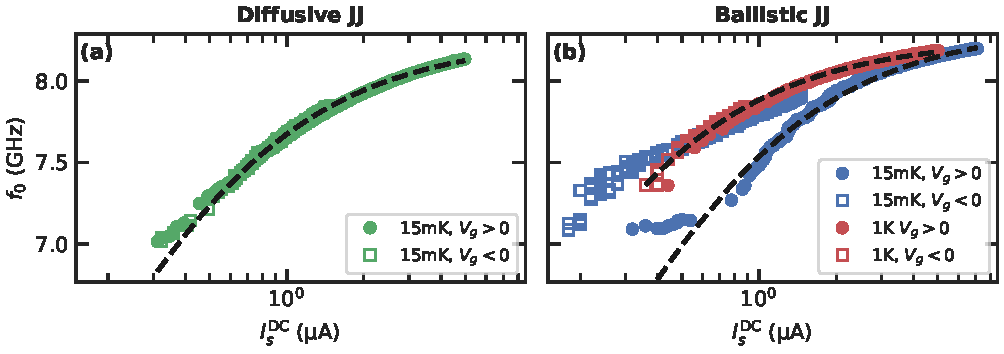
\includegraphics[width=\linewidth]{chapter-gJJ-CPR/figs/Figure2}
	\caption{
		\textbf{Evidence for non-sinusoidal CPR from deviation between Josephson inductance and critical current.}
		%
		MW-extracted $L_J$ versus DC-measured $I_c$ for the diffusive device at \SI{15}{\milli\kelvin} \textbf{(a)} and the ballistic one at \SI{15}{\milli\kelvin} and at \SI{1}{\kelvin} (\textbf{(b)}, blue and red, respectively).
		%
		Full circles (empty squares) correspond to $V_g>V_{\rm CNP}$ ($V_g<V_{\rm CNP}$).
		%
		Dashed line corresponds to an $L_J$ calculated from $I_c$ assuming a sinusoidal CPR.
		%
		Values of $L_J$ below the dashed line are due to current noise (see main text).
	}
	\label{fig:figure2}
\end{figure}

\textbf{TODO!!!! No fitting, but we calibrated fr,Lr! And we also don't calculate Ic, but extract LJ}

Assuming a purely sinusoidal current-phase relation, the Josephson inductance can be extracted from the current phase relation via $L_J = \hbar/(2\pi I_c \cos\delta)$.
%
However, depending on the exact shape of the CPR, $L_J$, and with it $f_0$, can significantly deviate from the above equations, cf. Supplementary Fig.~\ref{fig:SMinfluence}.
%
This leads to a reduced slope of the CPR around zero phase, which enhances $L_J$ compared to the case of a sinusoidal CPR for the same value of $I_c$.

Instead of relying only on the DC measured values of $I_c$ and the assumption of SIS CPR, we can directly extract $L_J$ from the MW measurement of $f_0$.
%
To calibrate the circuit parameters, we use additional measurements of reference devices shorted to with an open and a short to ground instead of a gJJ (see Supplementary Material Sec.~\ref{sec:SMcalibration} for details).
%
From this, we extract $f_{\lambda/2}=\SI{8.364}{\giga\hertz}$ and $L_r=\SI{3.671}{\nano\henry}$, which allows us to extract $L_J$ via Eq.~\ref{eq:Pogorzalek}.

In Fig.~\ref{fig:figure2}, we plot the observed Josephson inductance together with the measured critical currents for the measured devices.
%
Regardless of diffusive or ballistic transport, or elevated temeperatures, we observe significant deviations from a sinusoidal CPR underlying $L_J(I_c)$.
%
For large values of $I_c$, we observe larger values for the measured Josephson inductance as expected from sinusoidal CPR, which points at a forward-skew of the CPR in line with Eq.~\ref{eq:CPR-ball}.
%
On the other hand, small critical currents seem to correspond to smaller Josephson inductances.
%
This could either be due to backwards skew in the CPR, or current noise, artificially reducing the measured value of $I_c$.
%
Backwards skew in gJJ is highly unlikely and has not been observed before, but current noise in our setups can have a significant influence.
%
As detailed in Supplementary Material Sec.~\ref{sec:SMfitbiascurrent}, we estimate low-frequency current noise to range between \SIrange{110}{390}{\nano\ampere} in the setups used for measuring the diffusive and ballistic device, respectively.
%
Added to the measured values of $I_c$, this amount of current noise would be sufficient to move all data points such that $L_J$ is larger than expected from sinusoidal CPR for all $I_c$, cf. Supplementary Fig.~\ref{fig:SMfigure2}.

Additionally, we can directly compare the estimates for the junction critical current from our DC measurement, $I_c$, with the value calculated from our MW measurement of the resonance frequency via Eq.~\ref{eq:LJsin}, $I_c^{\rm MW}=I_c\left(L_J\left(f_0\right)\right)$. 
%
As shown in Fig.~\ref{fig:figure3}, our devices exhibit tunable supercurrent over almost two orders of magnitude range.
%
In the diffusive device, $I_c$ and $I_c^{\rm MW}$ match closely, but small deviations at the low and high end are visible, with $I_c^{\rm MW}$ resulting in values larger than expected from DC.
%
Similarly, the DC measurements of the ballistic device at \SI{1}{\kelvin} underestimate the critical current as extracted from MW for small values of $I_c$, but match remarkably well everywhere else.
%
This matches with the expectation of reduced forward skewing of the CPR at higher temperatures:
%
The skew is due to the phase coherence of Andreev bound states traversing the normal region between the superconducting banks multiple times (or, in a similar picture, multiple ABS crossing the normal region) which in turn means a longer phase coherence length is required to keep this contribution.
%
As the phase coherence length is highly sensitive to temperature, an increase in the latter results in both a reduction of switching current and forward skewing~\cite{fuechsleEffectMicrowavesCurrentPhase2009,hagymasiJosephsonCurrentBallistic2010,black-schafferStronglyAnharmonicCurrentphase2010,rakytaMagneticFieldOscillations2016,englishObservationNonsinusoidalCurrentphase2016}.
%
At base temperature, the ballistic device deviates significantly from the DC-calculations, especially at low currents and $V_g<0$.
%
Deviations at large $I_c$ are less obvious, presumably due to the fact that in this regime, $L_J \ll L_r$ and the Josephson inductance has only minor effect on $f_0$.

At first glance, any forward skew in the CPR should lead to a drop in CPR slope.
%
Therefore, for the same value of $I_c$, $L_J$ should increase and $I_s^{\rm MW}<I_c$.
%
However, our fit results in the opposite behavior:
%
The fit model returns a larger $I_c$ than expected for a sinusoidal CPR, given that the data to be fitted has an underlying forward-skewed CPR.
%
This is achieved by returning incorrect values for $f_{\lambda/2}$ and $L_r$ which explains to mismatching values from Fig.~\ref{fig:figure2}.
%
In lack of a reference device with a simple short to ground instead of a gJJ, or a JJ with known sinusoidal CPR, we need additional measurements to accurately determine the CPRs of our devices.
%
This shows that extrapolation of a value for $L_J$ at microwave frequencies from DC measurements can lead to severe discrepancies.
%
In order to examine the underlying mechanisms further, we continue by studying the power and bias current dependence of our circuit.



\section{Reconstructing the current phase relation}

\subsection{Anharmonicity of a gJJ MW circuit}

The nonlinear inductance of a Josephson junction consequently introduces nonlinear behavior of the overall circuit.
%
Depending on the exact circuit design and participation ratio between Josephson and total circuit inductance, this nonlinearity is more or less diluted, yet finite so-called anharmonicity $\beta$, i.e. deviation from the ideal case of pure LC-resonator behavior, remains.
%
Our circuit architecture allows us to extract this quantity directly and to calculate the expected CPR skew.

We can observe the anharmonicity of our DC bias circuit terminated with the diffusive gJJ by performing $S_{11}$ measurements at high drive powers for a series of different gate voltages, as shown in Fig.~\ref{fig:figure3} for $V_g=\SI{+10}{\volt}$.
%
At very low drive powers, $\beta$ has negligible effect on the circuit response, which can still be described by a purely harmonic oscillator here.
%
With increasing on-chip power $P_{\rm in}$, the resonance frequency experiences a down-shift, and both amplitude and phase of $S_{11}$ start to get skewed towards lower frequencies.
%
Once $P_{\rm in}$ exceeds a critical threshold, the resonator response bifurcates, which can be seen by the discontinuity in the data.
%
For reference, all other measurements of this device were performed at $P_{\rm in}\approx\SI{-131.4}{dBm}$, still in the linear regime and with a maximum current at the junction of $I_{\rm MW}\approx\SI{3.0}{\nano\ampere}$ well below the critical current, cf. Supplementary Material Fig.~\ref{fig:SMFigpoweratJJ}.

Using the previously determined parameters $f_0$, $\kappa_i$ and $\kappa_e$, we can model the data by solving the equation of motion of a harmonic oscillator with an additional third order term in the cavity field with amplitude $\beta$, 
%
\begin{align}
\dot{\alpha} = \left[ -i \left( \Delta+\beta\abs{\alpha}^2 \right)-\frac{\kappa}{2} \right]\alpha + \sqrt{\kappa_\text{e}} S_\text{in}\ ,
\label{eq:Duffing-EOM}
\end{align}
%
where $S_\text{in}$ is the field amplitude of the drive, $\Delta$ the frequency detuning and $\kappa=\kappa_i+\kappa_e$, as detailed in Supplementary Material Sec.~\ref{sec:SMduffing}.


Best agreement between data and model is reached when introducing nonlinear dissipation in the form of increasing internal linewidth that grows with the square root of the drive power, $\delta\kappa_i/\kappa_i(0)=\gamma \sqrt{P_{\rm in}}$, cf. Supplementary Section~\ref{sec:SMduffing} and Supplementary Figs.~\ref{fig:SMpower} and \ref{fig:SMFig-lossrates-power}.
%
This is in contrast with circuits incorporating standard aluminum oxide JJs, where nonlinear dissipation with increasing power is usually absent~\cite{boakninDispersiveMicrowaveBifurcation2007b}.

\begin{figure}[t]
	\centering
	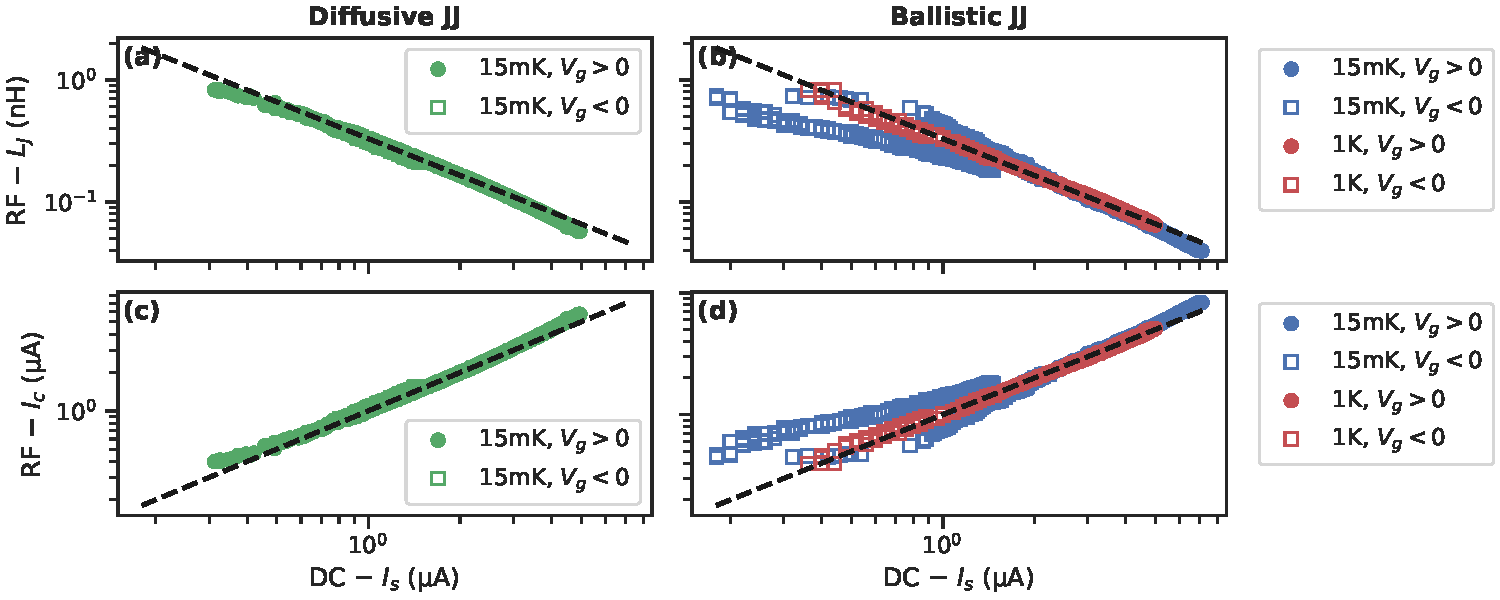
\includegraphics[width=\linewidth]{chapter-gJJ-CPR/figs/Figure3}
	\caption{
		\textbf{Extracting the anharmonicity coefficient.}
		%
		\textbf{(a)} Absolute value of the reflection coefficient $S_{11}$ versus frequency for increasing drive power.
		%
		Due to the circuit nonlinearity, the resonator experiences a downshift and bifurcation at elevated drive powers.
		%
		Solid lines indicate linecuts in \textbf{(b)} and \textbf{(c)}.
		%
		\textbf{(b-c)} Absolute value \textbf{(b)} and phase \textbf{(c)} of $S_{11}$ for varying drive power as indicated in \textbf{(a)}.
		%
		Linecuts are each offset by $-0.5$ in y for clarity.
		%
		Black lines are fits.
		%
		\textbf{(d)} Anharmonicity coefficient vs gate voltage.
		%
		Black dots: data as extracted from fits as in \textbf{(b-c)}, blue line: model using $I_c$ and assuming sinusoidal CPR, orange line: model using $L_J$.
	}
	\label{fig:figure3}
\end{figure}

There are several dissipation mechanisms known in superconducting microwave circuits that depend on drive power, such as on-chip heating~\cite{portisPowerinducedSwitchingHTS1991,heinFundamentalLimitsLinear1997,wosikPowerHandlingCapabilities1997}, dielectric losses~\cite{martinisDecoherenceJosephsonQubits2005c,oconnellMicrowaveDielectricLoss2008a,gunnarssonDielectricLossesMultilayer2013,lisenfeldElectricFieldSpectroscopy2019}, or subgap losses~\cite{dassonnevilleDissipationSupercurrentFluctuations2013,ferrierPhasedependentAndreevSpectrum2013,dassonnevilleCoherenceenhancedPhasedependentDissipation2018}.
%
Heating of the circuit itself is unlikely since $f_0$ should tune significantly stronger due to a reduced $I_c$ at elevated temperatures, with potentially significant influence on $f_0$, c.f. Fig.~\ref{fig:figure1}, which we did not observe for any of the gate voltages.
%
Moreover, the power dissipated on-chip is extremely small and very unlikely to cause even local heating.

Losses due to electric dipole moments of two-level systems are also unlikely the source of observation, as these are known to be activated for decreasing drive excitation voltages~\cite{martinisDecoherenceJosephsonQubits2005c,oconnellMicrowaveDielectricLoss2008a,gunnarssonDielectricLossesMultilayer2013}.
%
Moreover, TLS mainly reside in disordered dielectric materials.
%
However, there is only dielectric volume present at the shunt capacitor dielectric and the gJJ (encapsulating BN and HSQ top-gate).
%
Here, the circuit has voltage nodes and voltage fluctuations, which could activate the TLS, are expected to have negligible effect on the circuit performance.

We therefore attribute the source of the observed nonlinear damping to low-lying subgap states within the induced superconducting gap in the gJJ.
%
These subgap states can be due to e.g. intransparent superconductor-normal contacts, or Andreev bound states with large transverse momentum, polluting the bulk superconducting gap and leading to microwave loss~\cite{schmidtBallisticGrapheneSuperconducting2018}.
%
As the drive power increases, these subgap states get populated, resulting in an internal loss rate that grows with the square root of the input power, cf. Supplementary Fig.~\ref{fig:SMFig-lossrates-power}.
%
Loss mechanisms in similar SNS systems, with normal metal weak links, have shown similar effects~\cite{fuechsleEffectMicrowavesCurrentPhase2009,dassonnevilleDissipationSupercurrentFluctuations2013}, but they have not been observed before in gJJ.

The $\beta$ term in Eq.~\ref{eq:Duffing-EOM} is due to the anharmonicity of the microwave cavity for high drive powers which is evident when expanding the Josephson energy potential to higher orders,
\begin{align}
V_J(\delta) \approx E_J \frac{\delta^2}{2} - E_J\left( 1-\frac{3\sum\tau_i^2}{4\sum\tau_i} \right) \frac{\delta^4}{24} +\mathcal{O}(\delta^6)\ , 
\end{align}
%
where $E_J=\Delta_0\sum\tau_i/4$~\cite{kringhojAnharmonicitySuperconductingQubit2018}.
%
In Fig.~\ref{fig:figure3}(d), we compare the measured value of the anharmonicity coefficient with the one expected from a CPW shorted to ground by a Josephson junction, approximately given by $p^3/2$ with the participation ratio between Josephson and total inductance $p=L_J/(L_r+L_J)$~\cite{wilsonPhotonGenerationElectromagnetic2010b,zhouHighgainWeaklyNonlinear2014}.



Surprisingly, assuming a sinusoidal CPR and using $I_c$ to calculate $L_J$ results in a closer match to the observed coefficient than the expected value as calculated from the Josephson inductance directly observed in Fig.~\ref{fig:figure2}.
%
\textbf{TODO!!! WHY IS THAT?}
%
Without knowing exactly how many ABS channels are active in the JJ, it is not possible to extract a number for $\tau$, as the measured anharmonicity coefficient only returns information on $\sum\tau_i=N\tau$.
%
Additional experiments, such as extracting the transparency for each channel from multiple Andreev reflection via voltage-biased measurements, would be required to reach further conclusions~\cite{scheerConductionChannelTransmissions1997,goffmanConductionChannelsInAsAl2017,bretheauTunnellingSpectroscopyAndreev2017a,pandeyAndreevReflectionBallistic2019}.


\subsection{Bias current dependence}

A second way of reconstructing the CPR is by means of analyzing the bias current dependence of the high frequency circuit response, as this allows for a direct measure of $L_J(I_b)$.
%
We model the bias current dependence of both the ballistic and diffusive device at \SI{15}{\milli\kelvin} using Eqs.~\ref{eq:LJgeneral} and \ref{eq:Pogorzalek} under the assumption of a general CPR according to Eq.~\ref{eq:CPR-ball} and using $\tau$ as a free parameter, as shown in Fig.~\ref{fig:figure4}(a).
%
For details on the fitting algorithm, see the Supplemental Material Sec.~\ref{sec:fitbiascurrent}.

Our model accurately reproduces the data for all measured gate voltages, cf. Fig.~\ref{fig:figure4}(a), which allows us to extract a CPR-transparency parameter $\tau(V_g)$, as plotted in Fig.~\ref{fig:figure4}
(b).
%
We extract an average channel transmission $\tau_{\rm diff}=0.60\pm0.10$ and $\tau_{\rm ball}=0.78\pm0.09$ for the diffusive and ballistic device, respectively, at base temperature.
%
Measurements at \SI{1}{\kelvin} were not performed.
%
The resulting CPRs are forward skewed, as plotted in Fig.~\ref{fig:figure4}(c).
%
With skew defined as the deviation of the CPR maximum from phase $\pi/2$, $S=2\delta_{\rm max}/\pi -1$, the corresponding values are $S_{\rm diff}=0.15\pm0.03$ and $S_{\rm ball}=0.26\pm0.07$ for the diffusive and ballistic device, respectively.
%
We note that this is comparable to the results obtained from DC-measurements of the CPR~\cite{englishObservationNonsinusoidalCurrentphase2016,nandaCurrentPhaseRelationBallistic2017}.

\textbf{TODO: UPDATE!!!}
We plot the thus reconstructed current phase relations of both the ballistic and diffusive gJJ in Fig.~\ref{fig:figure4}(c).
%
While the relatively small forward skew of the diffusive device only deviates slightly from the case of a perfectly sinusoidal CPR, the ballistic device shows significant forward skewing.
%
We would like to point out that even though the skew in the diffusive case is only minor, our MW circuit still sensitive enough to these small changes, making its use competitive with DC-measurements of the CPR by using asymmetric SQUIDs or pickup loops.

\begin{figure}[t]
	\centering
	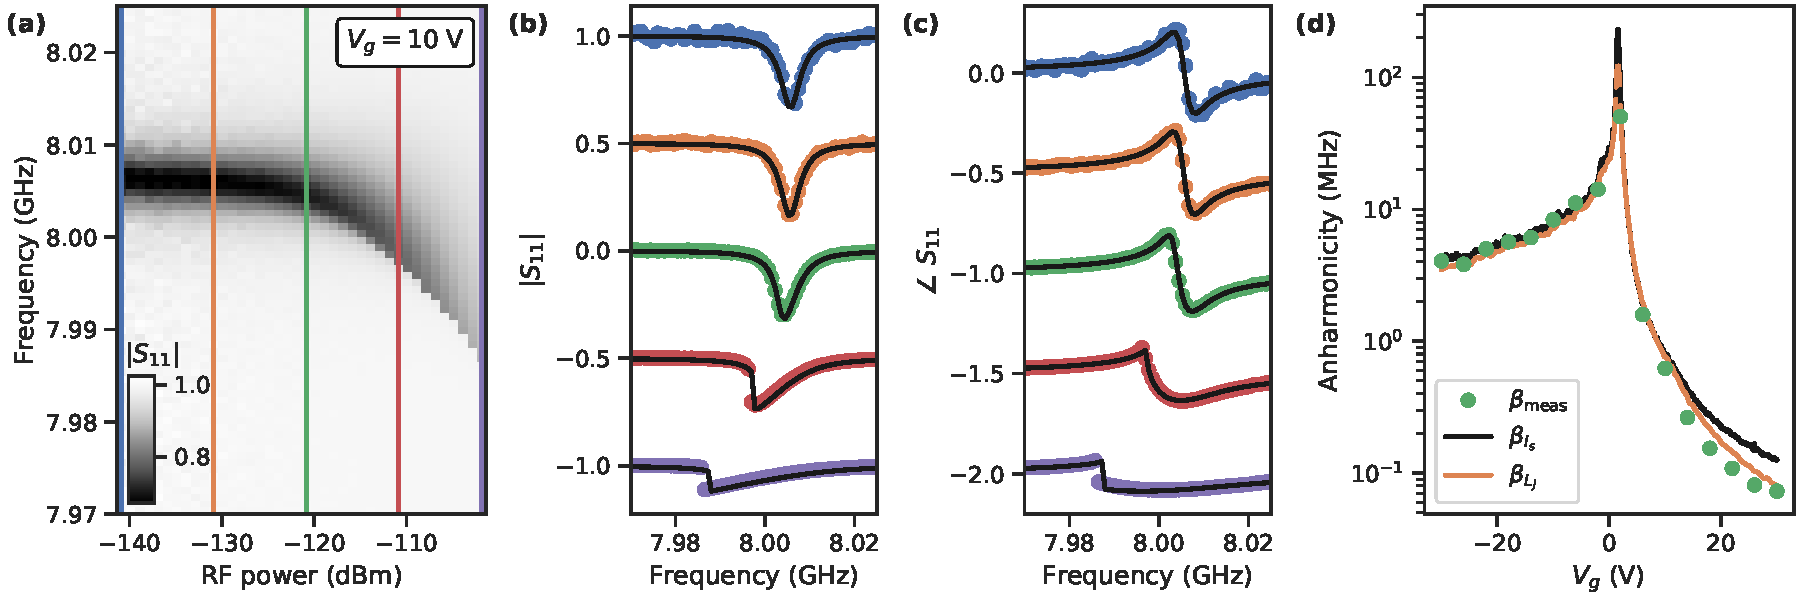
\includegraphics[width=\linewidth]{chapter-gJJ-CPR/figs/Figure4}
	\caption{
		\textbf{Observation of the skewness of the current phase relation by measuring the DC current dependence of the linear response of the Josephson inductance.}
		%
		Fitting the bias current dependence \textbf{(a)}, we can extract the junction transparency \textbf{(b)} and corresponding CPR skew \textbf{(c)} for the diffusive (green) and ballistic (blue) gJJ device versus gate voltage.
		%
		\textbf{(d)} Reconstructed current-phase relation for the diffusive (green) and ballistic (blue) device.
		%
		The large transparency of the ballistic JJ leads to significant forward skewing, while the relatively low transparency of the diffusive JJ only results in minor skewing.
	}
	\label{fig:figure4}
\end{figure}

\section{Conclusion}

We were able to reconstruct the CPR of gJJs by embedding the latter in superconducting microwave circuits.
%
Our results show that scattering of charge carriers, as well as elevated temperature, reduce the CPR skew and with it the circuit anharmonicity via the change in nonlinearity of the JJ itself.
%
Our circuit architecture is an attractive candidate for analyzing the CPR of exotic JJs, such as ferromagnetic or topological ones~\cite{golubovCurrentphaseRelationJosephson2004a,sochnikovNonsinusoidalCurrentPhaseRelationship2015,stoutimoreSecondHarmonicCurrentPhaseRelation2018,assoulineSpinOrbitInducedPhaseshift2019,muraniMicrowaveSignatureTopological2019}.
%
Moreover, the influence of high microwave powers on the CPR can be studied straightforwardly, as this only requires repeating the bias current measurements at various powers.
%
Additionally, the combination of bias current and power dependence should allow to trace out a larger part of the CPR than just around zero phase.
%
Finally, on top of a built-in method of reconstructing phase-sensitive information, incorporating asymmetric gate-tunable SQUIDs instead of single JJs would enable a further in-situ method of probing and reconstructing the CPR.

For the case of graphene Josephson junctions in cQED applications, they seem rather impractical for relatively high-power devices such as quantum-limited parametric amplification, as the inherent nonlinear damping due to the subgap states limits the maximum drive power.
%
Future research on improvements towards a hard superconducting gap could advance these applications.
%
Nevertheless, using gJJs in low-power circuits, such as transmon qubits, is still an attractive alternative to the established aluminum oxide JJs, as the gate-tunability and potential sweet spots in the Fabry-Pérot regime could allow for long qubit coherence times.
%
Our results also indicate that scattering mechanisms, such as diffusive transport or higher temperatures, inside of semiconducting JJs in MW circuits could even be beneficial for cQED because the increased circuit anharmonicity could result in more coherent circuits.

%%%%%%%%%%%%%%%%%%%%%%%%%%%%%%%%%%%
% Insert SM.tex contents here

\clearpage
\pagebreak

%\widetext

%\setcounter{equation}{0}
%\setcounter{figure}{0}
%\setcounter{table}{0}
%\setcounter{page}{1}
%\setcounter{section}{0}

%\renewcommand{\thepage}{S\arabic{page}}
%\renewcommand{\thesection}{S\Roman{section}}
%\renewcommand{\thetable}{S\Roman{table}}
%\renewcommand{\thefigure}{S\arabic{figure}}
%\renewcommand{\theequation}{S\arabic{equation}}
%\renewcommand{\bibnumfmt}[1]{[S#1]}
%\renewcommand{\citenumfont}[1]{S#1}

\section{Supplementary Material: Current phase relations of graphene Josephson junctions in microwave circuits}\label{sec:SM}

\subsection{Classification as diffusive or ballistic JJ}\label{sec:SMballistic}

As stated in the main text, we define the device as ballistic or diffusive in the presence or absence of Fabry-Pérot-like oscillations.
%
In Fig.~\ref{fig:SMFig-ballistic}, we plot these oscillations after removing a third order background from the data to remove the overall gate-voltage tuning dependence.
%
Both at base temperature and at \SI{1}{\kelvin}, we observe high-frequent, highly correlated oscillations in all off $f_0$, $I_c$ and $G_n=R_n^{-1}$ for the \textit{ballistic} device, which justifies its classification as such.
%
The oscillation period allows an estimate of a cavity length of \SI{390}{\nano\meter} for the ABS inside the JJ~\cite{schmidtBallisticGrapheneSuperconducting2018}.
%
For the same voltage range, however, the \textit{diffusive} device only shows a low-frequent trend originating from the deviation about the removed background, thus lacking the ballistic feature.

\begin{figure}[!h]
	\centering
	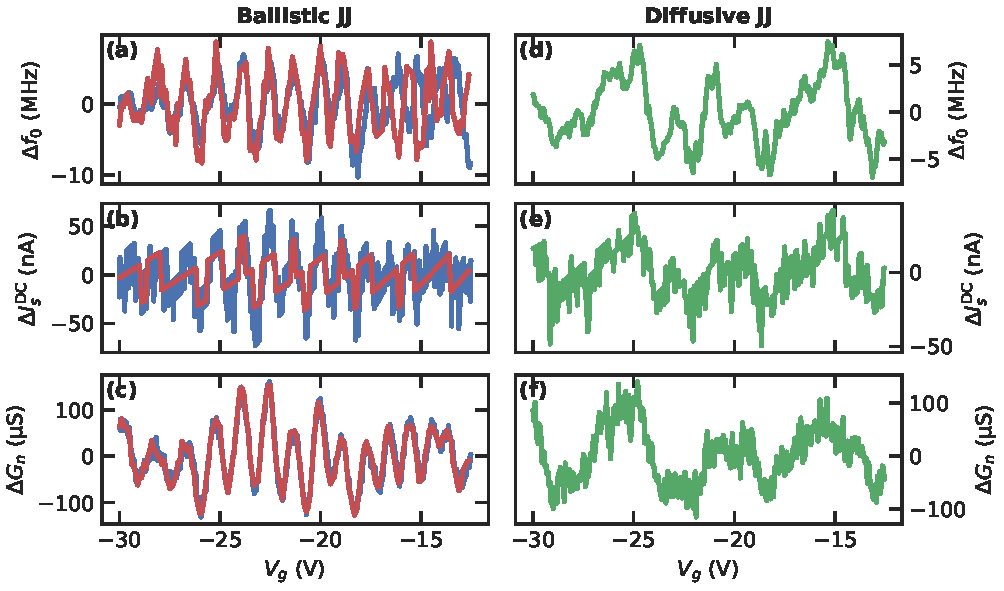
\includegraphics[width=\linewidth]{chapter-gJJ-CPR/figs/SMFigure-ballistic}
	\caption{
		\textbf{Fabry-Pérot oscillations in the ballistic device.}
		%
		\textbf{(a-c)} Oscillations in the resonance frequency, DC-switching current and normal state conductance as a function of gate voltage for the ballistic device at base temperature (blue) and \SI{1}{\kelvin} (red).
		%
		\textbf{(d-f)} For the diffusive device, no such features are observed, only a slowly varying background, justifying the classification as \textit{diffusive} device.
	}
	\label{fig:SMFig-ballistic}
\end{figure}



\subsection{Estimation of the fridge attenuation}\label{sec:SMattenuation}

We can estimate the attenuation of our MW input line by using the cryogenic HEMT as a calibrated noise source.
%
The HEMT noise power is given by
%
\begin{align}
P_{\rm HEMT}=10\log\left(\frac{k_B T_{\rm HEMT}}{\si{\milli\watt}}\right) + 10\log\left(\frac{\Delta f}{\si{\hertz}}\right)\ ,
\label{eq:HEMT}
\end{align}
%
with the Boltzmann constant $k_B$, the noise temperature of the HEMT $T_{\rm HEMT}=\SI{2}{\kelvin}$ as specified by the manufacturer and the measurement bandwidth $\Delta f=\SI{100}{\hertz}$.
%
The resulting noise power is $P_{\rm HEMT}=\SI{-175.59}{dBm}$.
%
Additionally, we can calculate the average background signal arriving at the VNA by averaging all $S_{11}$ traces in the areas off-resonant to the cavity, which leaves the background unaltered in power.
%
Doing so, we extract an average signal and standard deviation, which yields the signal-to-noise ratio at the VNA, $\text{SNR}_\text{VNA}=\SI{43.85}{\decibel}$, for a VNA output power of \SI{-20}{dBm}.
%
Assuming \SI{2}{\decibel} of cable loss between sample and HEMT, we arrive at an attenuation of \SI{111.74}{dB} of our VNA input line,

\subsection{Extraction of $I_c$ and $f_0$}\label{sec:SMextraction}

The DC switching current (Fig.~\ref{fig:figure1}(b,c)) is taken as the current at which $\partial V/\partial I_b$ is maximum, where $V$ is the measured voltage drop across the JJ.
%
Noise or interference on the DC lines could lead to a reduction of the measured $I_c$ compared to the true value.
%
To get a more accurate estimation of $I_c$ together with a good understanding of the noise sources, switching histograms are the preferred measurement method.
%
The necessary setup was however not available at the time of measurement.

To extract resonance frequency and loss rates from the MW data, we fit the reflection coefficient to the following model (cf. Ref.~\cite{bosmanBroadbandArchitectureGalvanically2015c} for a derivation):
%
\begin{align}
S_{11}(\omega) = -1+\frac{2\kappa_e}{\kappa+2i\Delta},
\end{align}
%
where $\kappa=\kappa_e+\kappa_i$ denoting the total, external and internal loss rates, respectively, and $\Delta=\omega-\omega_0$ with resonance frequency $\omega_0=2\pi f_0$.
%
The measured $S_{11}$ is usually distorted by a setup-related microwave background of the following shape:
\begin{align}
B(\omega) = \left(a+b\omega+c\omega^2\right)e^{i\left(a^\prime+b^\prime\omega\right)},
\end{align}
%
and with additional rotation by angle $\theta$ in the complex plane, the measured $S_{11}^\prime$ is:
\begin{align}
S_{11}^\prime(\omega)=B(\omega)\left(e^{i\theta}\left(S_{11}(\omega)+1\right)-1\right)
\end{align}
%
The origin of the microwave background and phase rotations are impedance mismatches in the wiring originating from various non-ideal circuit elements (e.g. connectors, attenuators, directional couplers, wirebonds).
%
Standing waves can form in some segments of the wiring which interfere with the measured signal, thus producing an oscillating measurement background.
%
To remove this background for the gate voltage sweeps (Fig.~\ref{fig:figure1}(d,e)), we pick the measurement trace at the CNP as the one with only background signal, as the MW resonance is extremely broad and effectively not present here.
%
We then divide the other traces by this trace, resulting in a much cleaner signal.
%
For measurements based on bias current sweeps, cf. Fig~\ref{fig:figure5}(a), we take the MW background as the $S_{11}$ trace at $I_b>I_s$.
%
Here, the JJ switched to the normal state and the MW resonance is not present in the measurement.
%
In order to remove MW background from the power dependence, we mask the regions in which there are resonances for the various powers and gate voltage setpoints, and average the remaining traces.
%
This way, we obtain a power and frequency map of the MW background, which we use for removing background signal from power traces, such as the one in Fig.~\ref{fig:figure3}(a).

\subsection{Extraction of $f_r$, $L_r$ and $L_J$}\label{sec:SMcalibration}

We can derive an expression for the circuit resonance frequency depending on the other parameters by using the impedances defined in Fig.~\ref{fig:rfderivation}.
%
The circuit impedance as seen from the JJ towards the CPW, $Z_1$, the input impedance as seen from the CPW towards the input port, $Z_2$, and the overall parallel circuit impedance $Z_q$ are:
%
\begin{align}
Z_1 &= Z_0 \frac{Z_2+Z_0\tanh\gamma l}{Z_0+Z_2\tanh\gamma l} \\
Z_2 &= \left(\frac{1}{Z_{C_s}}+\frac{1}{Z_0}\right)^{-1} = \left(i\omega C_s+\frac{1}{Z_0}\right)^{-1} \\
Z_q &= \left(\frac{1}{Z_{J}}+\frac{1}{Z_1}\right)^{-1} = \left(\frac{1}{i\omega L_J}+\frac{1}{Z_1}\right)^{-1}\ ,
\end{align}
%
with the CPW length $l$, the complex CPW loss per unit length $\gamma=\alpha+i\beta$, and the transmission line impedance $Z_0$.
%
Note that the junction impedance $Z_J$ can be further extended by an RCSJ model and should include additional capacitance for the gate and inductance for the contact electrodes, as described in Ref.~\cite{schmidtBallisticGrapheneSuperconducting2018}.
%
Assuming negligible losses in the CPW on resonance, $\gamma l\approx i\beta l = i\pi\omega_0/\omega_r$, i.e. the CPW only acts as a phase shifter.
%
The resonance condition of the above circuit is for the imaginary part of the admittance $Y=1/Z_q$ to be zero, which yields
%
\begin{align}
0 = \Im \left[ \frac{1}{i\omega_0 L_J} + \frac{1}{Z_0}\frac{Z_0+iZ_2\tan\left(\pi\omega_0/\omega_r\right)}{Z_2+iZ_0\tan\left(\pi\omega_0/\omega_r\right)}\right]
\label{eq:SolAnalytical}
\end{align}
%
%The solution of this equation for $\omega_0$ is plotted as solid line in Fig.~\ref{fig:SMval}(a).
%
We can approximate the above by a similar method as the authors of Refs.~\cite{wallquistSelectiveCouplingSuperconducting2006a,wustmannParametricResonanceTunable2013,pogorzalekHystereticFluxResponse2017}:
%
Assuming a large shunt capacitance at the input, such that $Z_2\approx 0$ and expanding the tangent, we arrive at the expression stated in Eq.~\ref{eq:Pogorzalek}.% which is plotted as dashed line in Fig.~\ref{fig:SMval}(a).
%
This assumption is justified since $C_s\approx\SI{27}{\pico\farad}$ for our devices, such that both $Z_2\approx \SI{0.2}{\ohm} \ll Z_0=\SI{50}{\ohm}$.
%
We find that for all values of $L_J$, including the range in our experiments, the approximation differs by less than \SI{0.2}{\percent} from the analytical solution (see below).


\begin{figure}
	\centering
	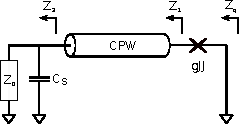
\includegraphics[width=0.5\linewidth]{chapter-gJJ-CPR/figs/rfderivation}
	\caption{
		\textbf{Derivation of resonance frequency.}
		%
		We define the three impedances $Z_1$, $Z_2$ and $Z_q$ as seen from the CPW towards the input port, from the gJJ towards the CPW, and as the parallel circuit impedance.
		%
		The gJJ can further be modeled via an RCSJ-model, and an additional gate capacitance (not shown, see text for details).
	}
	\label{fig:rfderivation}
\end{figure}


We extract the circuit parameters from our measurement data in the same fashion as described in the Supplementary Material of Ref.~\cite{schmidtBallisticGrapheneSuperconducting2018}:
%
In short, we use a reference device with no junction at the end to calibrate $f_r$ and $L_r$, a reference device shorted to ground to calibrate the transmission line losses, and finite-element simulations to deduce additional inductances and capacitances of the leads and gate electrode.
%
This allows us to extract the Josephson inductance directly from the observed resonance frequency, regardless of the underlying CPR.
%
As shown in Fig.~\ref{fig:SMFigure-f0vsIcvsLj}, while there are significant deviations of Eq.~\ref{eq:Pogorzalek} to the measured $f_0(I_c)$, all measured devices fall on a single curve when plotted as a function of $L_J$, which verifies this approximation.

\begin{figure}
	\centering
	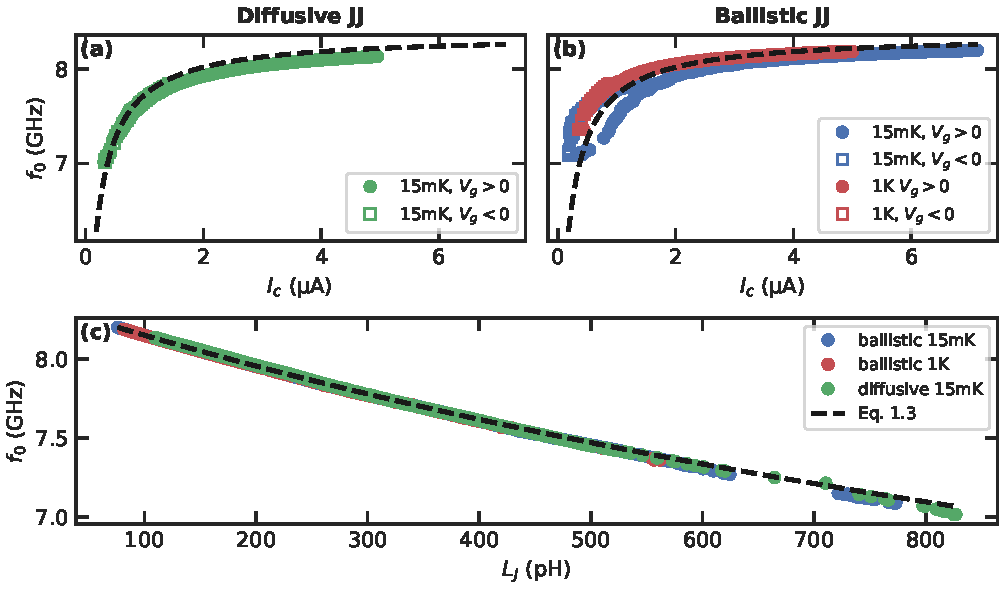
\includegraphics[width=\linewidth]{chapter-gJJ-CPR/figs/SMFigure-f0vsIcvsLj}
	\caption{
		\textbf{Resonance frequency vs switching currents for two different gJJ devices.}
		%
		Both the diffusive device at low temperature \textbf{(a)} and the ballistic device at \SI{1}{\kelvin} (\textbf{(b)}, red) show monotonically increasing $f_0$ versus DC-extracted switching currents.
		%
		In contrast, for low temperatures, the ballistic gJJ (\textbf{(b)}, blue) exhibits multi-valued $f_0\left(I_s\right)$ for gate voltages larger (full circles) and smaller (empty squares) than the charge neutrality point.
		%
		The	multivalued behavior in the ballistic device at low temperature presumably originates from significant differences in junction transparency between n- and p-doping, and only allows for a fit for $V_g>0$.
		%
		This is not observed at higher temperature or for the diffusive device.
		%
		Dashed lines correspond to Eq.~\ref{eq:Pogorzalek} under assumption of sinusoidal CPR.
		%
		\textbf{(c)} Resonance frequency as a function of observed Josephson inductance, showing good matching to Eq.~\ref{eq:Pogorzalek}.
	}
	\label{fig:SMFigure-f0vsIcvsLj}
\end{figure}

\subsection{Device response to drive power}\label{sec:SMduffing}

Following the method described in Ref.~\cite{schmidtCurrentDetectionUsing2020}, the equation of motion of the amplitude field $\alpha(t)$ of a resonator with weak anharmonicity $\beta$ written in the frame rotating with the drive $S_{\rm in}$ is given by Eq.~\ref{eq:Duffing-EOM}, from which the steady-state solution $\partial\alpha_0/\partial t=0$ results in the polynomial function
% 
\begin{align}
\beta^2 \alpha_0^6 + 2\Delta\beta\alpha_0^4 + \left(\Delta^2+\frac{\kappa^2}{4}\right)\alpha_0^2 - \kappa_\text{e} \abs{S_{\rm in}}^2 = 0\ ,
\label{eq:polynom}
\end{align}
%
which we can solve and use to calculate the expected reflection coefficient as our model,
\begin{align}
S_{11}=-1-\frac{\sqrt{\kappa_e}}{S_{\rm in}}\alpha_0\ .
\label{eq:S11anh}
\end{align}
%
to fit the measurement data.
%
We reduce the number of free parameters of this function from five to two by fixing $\omega_0$ and $\kappa_e$ as the values extracted at lowest drive power and calculating $S_{\rm in}$ from the fridge attenuation, see Supplementary Section Sec.~\ref{sec:attenuation}.
%
The remaining parameters are $\beta$ and $\kappa_i$, where the internal loss rate can in fact depend on the drive power, $\kappa_i=\kappa_i(S_{\rm in})$.
%
Fixing the loss rate to be constant throughout the fit does not lead to a good fit to the data, as shown in Fig.~\ref{fig:SMpower}.
%
Our algorithm first fits the measured data to return constant $\beta$ and $\kappa_i$, and uses these as initial values for a fit to extract the power dependent loss rate.

\begin{figure}
	\centering
	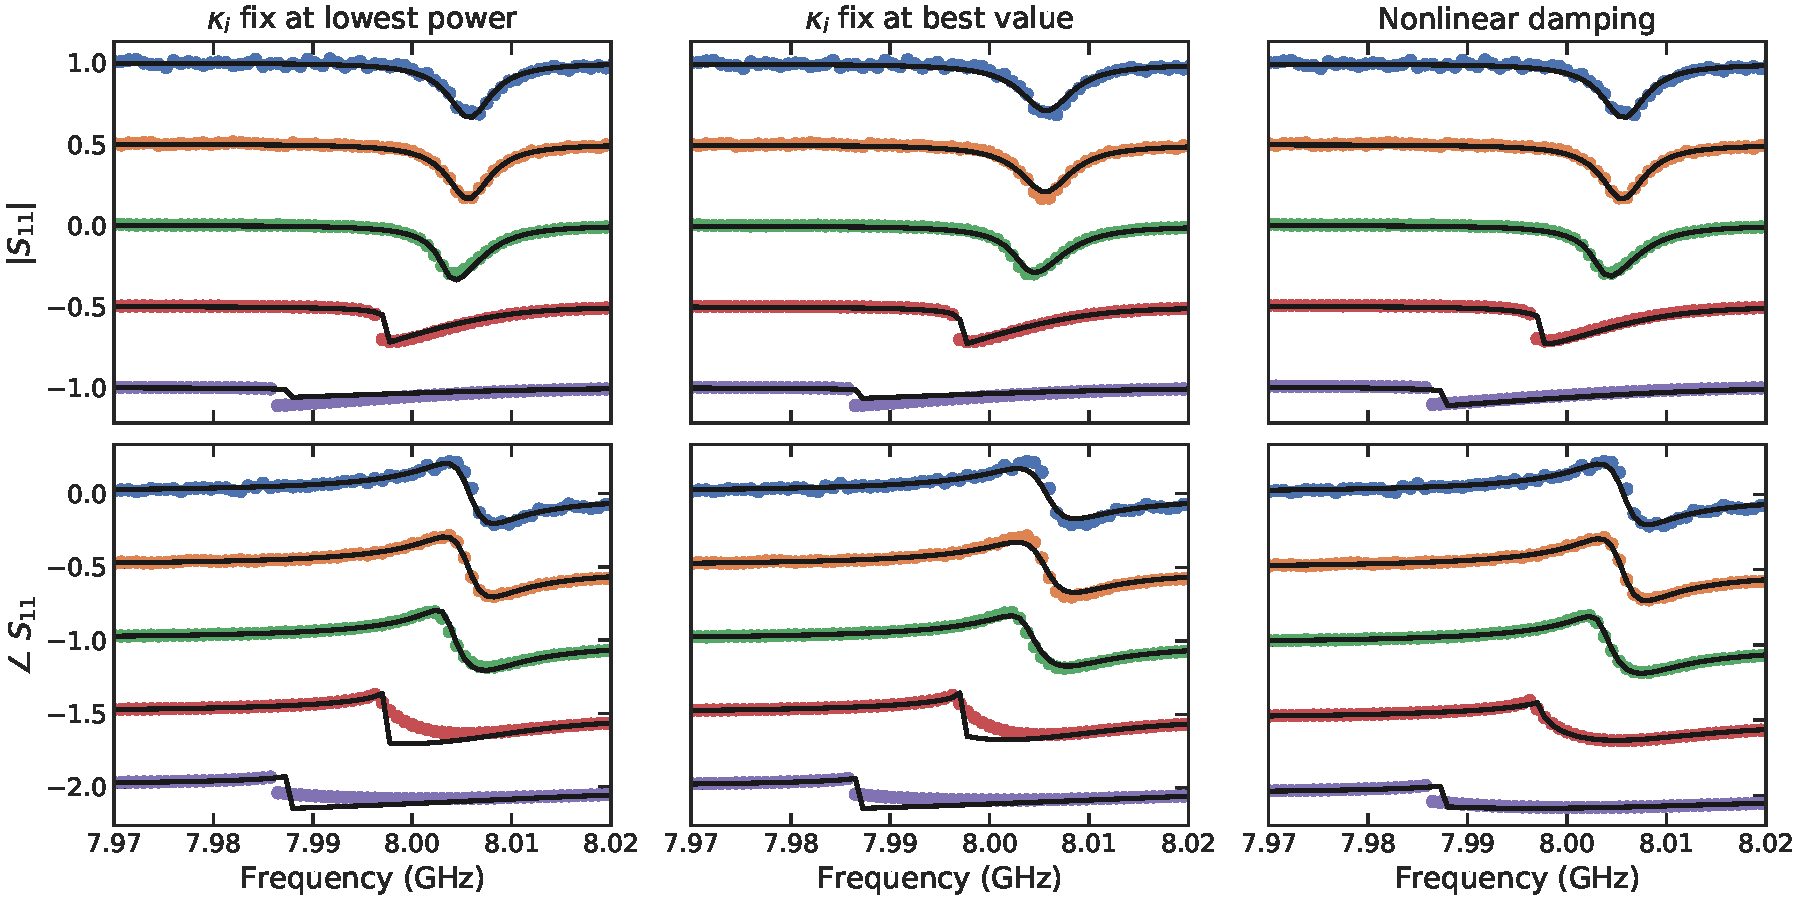
\includegraphics[width=\linewidth]{chapter-gJJ-CPR/figs/SMFigure-power}
	\caption{
		\textbf{Anharmonicity fit assuming different cases for $\kappa_i$.}
		%
		Fixing $\kappa_i$ to be the value at lowest drive power (first column) results in significantly worse fit than introducing it as constant, but free parameter (second column).
		%
		However, best agreement between data and model is reached when introducing nonlinear damping (third column and Fig.~\ref{fig:figure4}).
		%
		Linecuts and colors correspond to the ones in Fig.~\ref{fig:figure4}.
	}
	\label{fig:SMpower}
\end{figure}

We can fit the thus extracted change in internal linewidth using a linear growth in drive field $S_{\rm in}$ or square-root dependence on drive power,
\begin{align}
\kappa_i=\kappa_i(0)\left(\gamma\sqrt{P_{\rm in}}+1\right)
\label{eq:kintfitpower}
\end{align}
as shown in Fig.~\ref{fig:SMFig-lossrates-power}(a).
%
This strongly suggests internal losses originating from sub-gap states populated by the drive field.
%
Over the range of measured gate voltages, the increase in loss is roughly constant, with slightly larger values for positive compared to negative gate voltages, cf. Fig.~\ref{fig:SMFig-lossrates-power}(b).

\begin{figure}
	\centering
	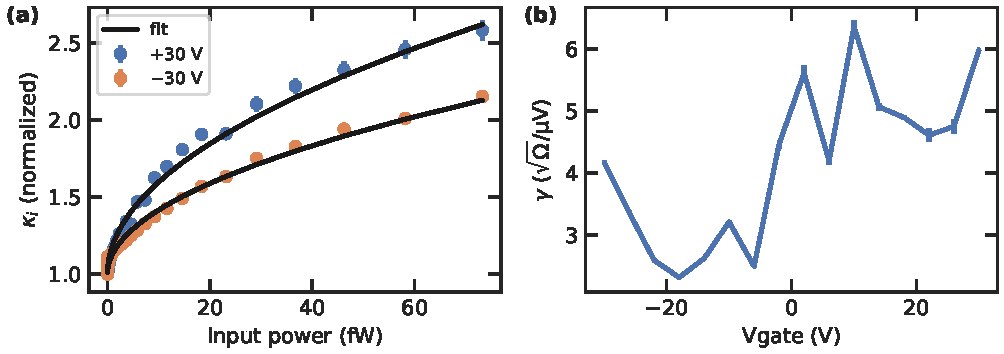
\includegraphics[width=\linewidth]{chapter-gJJ-CPR/figs/SMFigure-lossrates-power}
	\caption{
		\textbf{Nonlinear damping in the gJJ.}
		%
		\textbf{(a)} The internal linewidth of the diffusive device grows with the square root of the input power, regardless of gate voltage.
		%
		\textbf{(b)} The extracted fit parameter $\gamma$ is slightly lower for p-doping compared to n-doping.
		%
		$\gamma$ is related to the subgap losses.
	}
	\label{fig:SMFig-lossrates-power}
\end{figure}

\subsection{Device response to bias current}\label{sec:SMfitbiascurrent}
\subsubsection{Increasing loss rate}
In addition to an increase in $\kappa_i$ for high drive powers as discussed in the main text, the internal loss rate of our circuit also depends on bias current.
%
We observe an increasing loss rate for increasing bias current, cf. Fig~\ref{fig:SMFig-lossrates-current}.
%
Possible origins of this phenomenon are low-frequency noise on the DC electronics, as this artificially widens the measured cavity resonance if the measurement time is greater than the inverse noise frequency.
%
Additionally, phase-slip events might occur at larger rates if the Josephson energy potential is tilted, as compared to zero bias current.

The current noise amplitude can be calculated in two ways:
%
As shown in Fig.~\ref{fig:SMFig-lossrates-current}(a), the reflected signal exhibits a double-peak for bias currents close to $I_c$, in addition to an increase in linewidth.
%
This strongly suggests low-frequency current noise, modulating the resonance about the fixed bias current faster than the measurement scan.
%
From the peak spacing and the measured responsitvity $G_1=\partial f_0/\partial I_b$, i.e. the change in resonance frequency versus bias current, we can compute the current noise as
\begin{align}
\Delta I_n = \frac{\Delta f_0}{\left( \frac{\partial f_0}{\partial I_b} \right)}
\label{eq:currnoise-a}
\end{align}
%
We estimate $\Delta I_n\approx\SI{270}{\nano\ampere}$ due to low-frequency noise for the ballistic device.
%
Similarly, the increase in total linewidth can be fitted as a linear function of $G_1$, resulting in an upper bound for the total corresponding bias current induced losses, cf. Fig.~\ref{fig:SMFig-lossrates-current}(b).
%
For the ballistic device, we extract a total corresponding current noise $I_n\approx\SI{390}{\nano\ampere}$ for the ballistic, and $I_n\approx\SI{110}{\nano\ampere}$ for the diffusive device.
%
This leads us to believe that the setup used for the ballistic device was better isolated against current noise than the one for the diffusive device.
%
Still, some contribution due to processes such as phase slip events is necessary to explain the excess noise obtained from the increase in total linewidth.

\begin{figure}
	\centering
	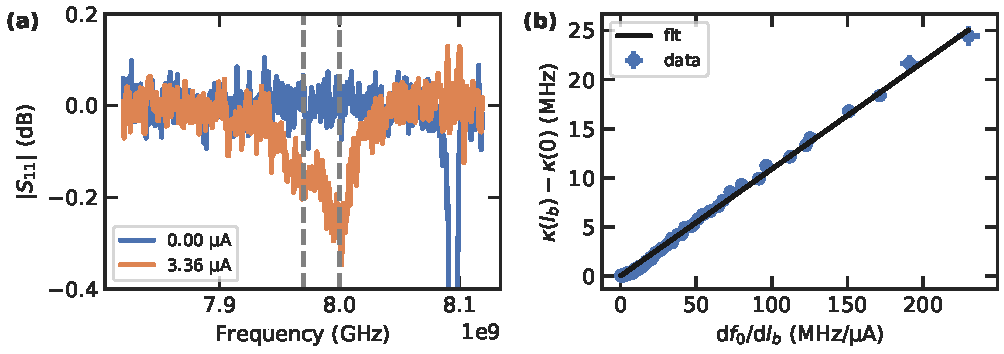
\includegraphics[width=\linewidth]{chapter-gJJ-CPR/figs/SMFigure-lossrates-current}
	\caption{
		\textbf{Internal loss rate for increasing bias current.}
		%
		Increasing loss rate with bias current could originate from either low-frequency noise or phase slip events.
	}
	\label{fig:SMFig-lossrates-current}
\end{figure}

Adding the estimates for $I_n$ to the measured $I_c$ of Fig.~\ref{fig:figure2} results in a rescaling of the current axis, cf. Fig.~\ref{fig:SMfigure2}

\begin{figure}
	\centering
	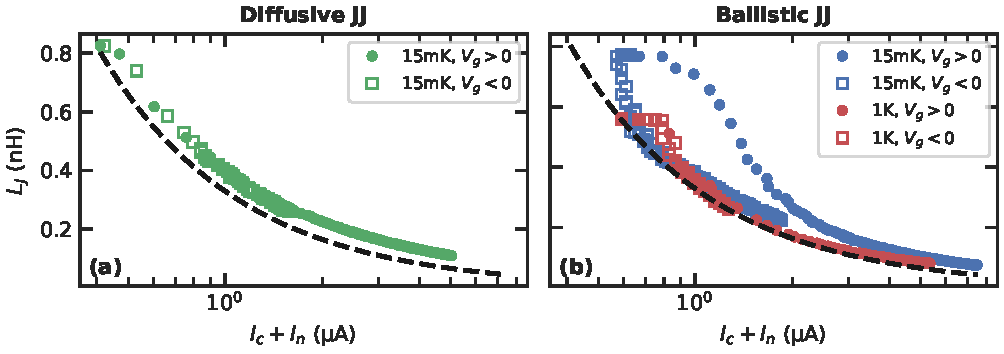
\includegraphics[width=\linewidth]{chapter-gJJ-CPR/figs/SMFigure2}
	\caption{
		\textbf{Josephson inductance and critical currents with added current noise.}
		%
		Accounting for $I_n=\SI{110}{\nano\ampere}$ for the diffusive \textbf{(a)} and $I_n=\SI{390}{\nano\ampere}$ for the ballistic device \textbf{(b)} results in all values of $L_J$ being larger than expected from a sinusoidal CPR (dashed line).
	}
	\label{fig:SMfigure2}
\end{figure}

\begin{figure}
	\centering
	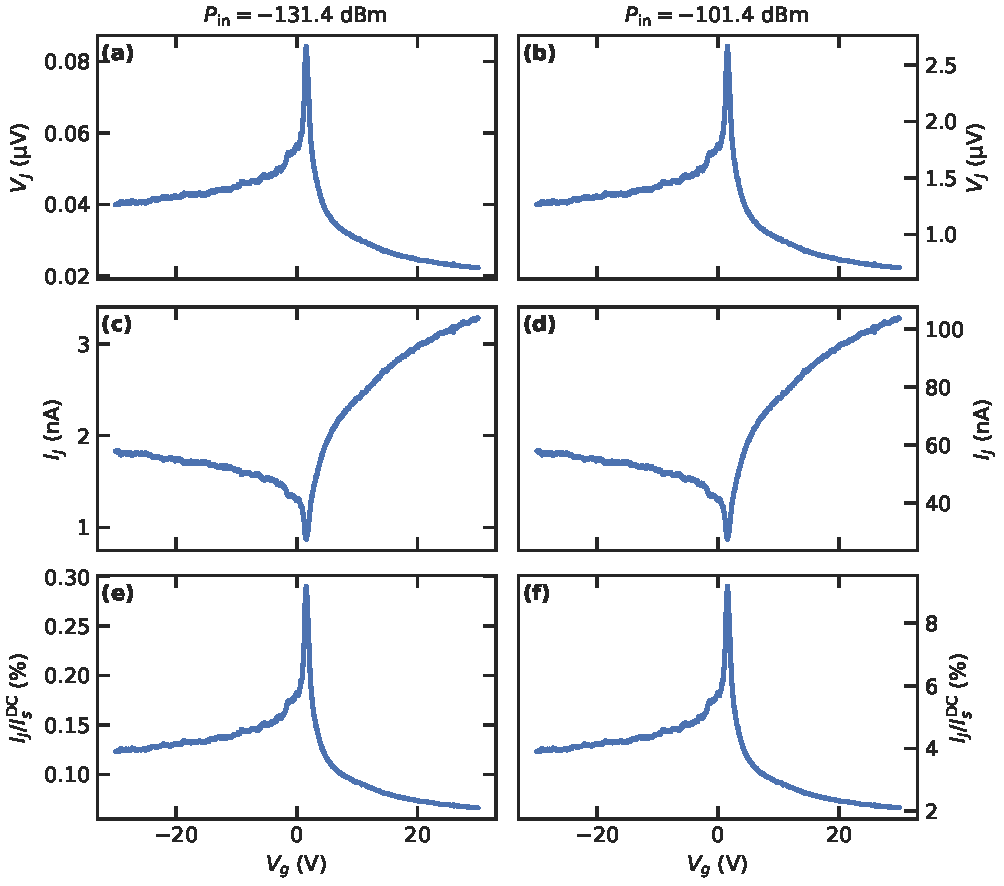
\includegraphics[width=\linewidth]{chapter-gJJ-CPR/figs/SMFigure-poweratJJ}
	\caption{
		\textbf{Voltage and current across the diffusive graphene Josephson junction.}
		%
		\textbf{(a,b)} Voltage across the JJ for varying gate voltage at reference power \textbf{(a)} and maximum drive power \textbf{(b)}.
		%
		\textbf{(c,d)} Current across the JJ for varying gate voltage at reference power \textbf{(c)} and maximum drive power \textbf{(d)}.
		%
		\textbf{(e,f)} Ratio of current across the JJ to DC-measured switching current for varying gate voltage at reference power \textbf{(e)} and maximum drive power \textbf{(f)}.
		%
		Note the different scales for the left and right column.
	}
	\label{fig:SMFigpoweratJJ}
\end{figure}

\begin{figure}
	\centering
	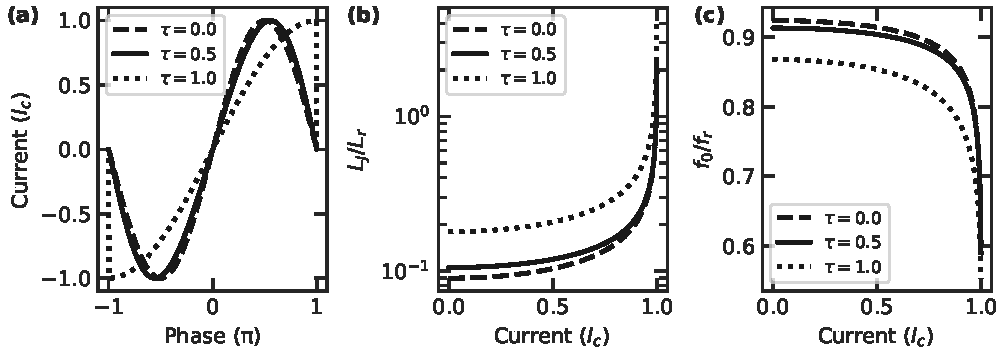
\includegraphics[width=\linewidth]{chapter-gJJ-CPR/figs/SMFigure-influence}
	\caption{
		\textbf{Predicted influence of the junction transparency on the bias current dependence.}
		%
		\textbf{(a)} CPR for various $\tau=0$ (solid), $\tau=0.5$ (dashed) and $\tau=1.0$	(dash-dotted).
		%
		\textbf{(b-c)} Josephson inductance \textbf{(b)} and resonance frequency \textbf{(c)} supercurrent for	same transparencies as in \textbf{(a)}.
		%
		Increased junction transmission leads to forward skewing of the CPR, thus a reduced slope and higher Josephson inductance, which in turn reduces the resonance frequency and increases the tuning.
	}
	\label{fig:SMinfluence}
\end{figure}

\subsubsection{Extracting $\tau$}
\textbf{TODO: REWRITE THIS BECAUSE WE NOW CALIBRATED FR AND LR!!!}
Without any knowledge on the junction transparency $\tau$, fitting data of a CPW cavity with JJ exhibiting a potentially nonsinusoidal CPR can lead to significant deviations from the true circuit parameters.
%
In Fig.~\ref{fig:SMtau}, we demonstrate the effect of $\tau$ on the extracted circuit parameters:
%
If the JJ shorting the CPW to ground has a forward skewed CPR, i.e. $\tau>0$, and Eq.~\ref{eq:Pogorzalek} is used to fit this data (dashed lines in Fig.~\ref{fig:SMtau}) under the assumption of a JJ with purely sinusoidal CPR, the extracted values (solid lines) for $f_r$ and $L_r$ will be too small compared with the true values, while $I_c$ will appear to be larger than expected, with consequently lower $L_J$.
%
Naively, one would assume the MW measurement to result in $L_J$ to be larger than the value expected from DC measurements due to the increased inverse CPR slope for identical $I_c$.
%
Nonetheless, the fit model accounting for the resonator tunability results in the opposite behavior.

To fit the bias current dependence data for extracting $\tau$, we first keep $\tau$ fixed and compare the fit residuals for various $\tau\in[0,1]$.
%
In a second step, we set $\tau$ as additional free parameter with the best results for $f_r$, $L_r$ and $I_c$, and set the initial value of $\tau$ as the one with previously determined minimum reduced $\chi^2$.
%
The fit converges more reliably than by setting $\tau$ as free parameter from the start, since this way the fit does not get trapped in a local minimum.

Both current and frequency noise, however, can result in artificial global minima in $\chi^2(\tau)$.
%
For a critical current of \SI{2}{\micro\ampere} and bias currents up to $0.9I_c$, already $\sigma_I\geq\SI{1}{\nano\ampere}$ is enough to significantly throw off the fit for low values of $\tau$.
%
Frequency noise of $\sigma_f<\SI{1}{\mega\hertz}$ has no influence on the fitting algorithm.
%
As the responsivity $\partial f_0/\partial I_b$ increases with $I_b$, so does the frequency noise for a fixed current noise.
%
From the average data fluctuations and comparing these with the expected $\sigma_f(\sigma_I)$, we estimate $\sigma_I<\SI{1}{\nano\ampere}$ in our setup.
%
We therefore conclude that our fitting algorithm should present a reliable way of extracting $\tau$. 

%\begin{figure}
%	\centering
%	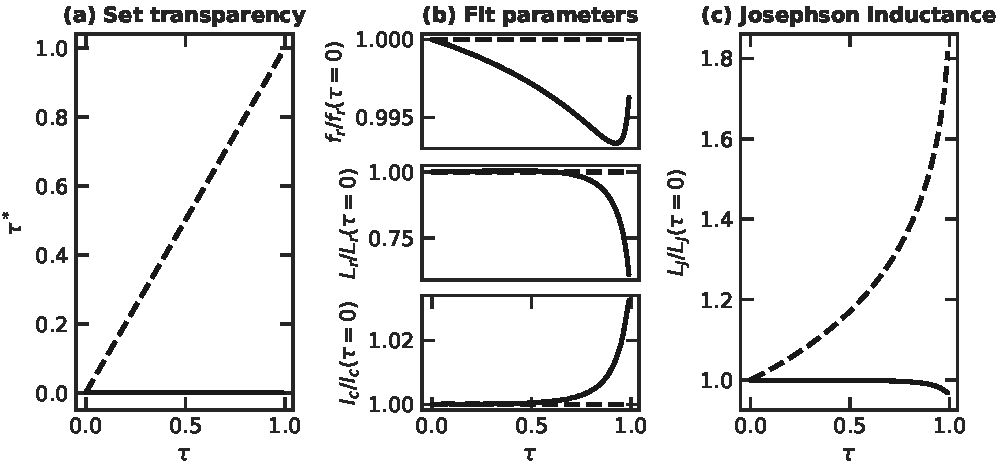
\includegraphics[width=\linewidth]{chapter-gJJ-CPR/figs/SMFigure-tauparams}
%	\caption{
%		\textbf{Influence of $\tau$ on extracted fit parameters with Eq.~\ref{eq:Pogorzalek}.}
%		Increasing $\tau$ (dashed line in \textbf{(a)}) results in a larger $L_J$ (dashed line in \textbf{(e)}), while the other fit parameters (dashed lines in \textbf{(b-d)}) remain constant.
%		%
%		In order for a fit model using Eq.~\ref{eq:Pogorzalek} under the assumption of a sinusoidal CPR (solid lines) to reproduce the data (points), significant deviations from the true parameters occur.
%		%
%		Specifically, the fit model returns a larger critical current than expected which leads to a reduced calculated $L_J$, even though the real $L_J$ increases with $\tau$.
%	}
%	\label{fig:SMtau}
%\end{figure}
%
%\begin{figure}
%	\centering
%	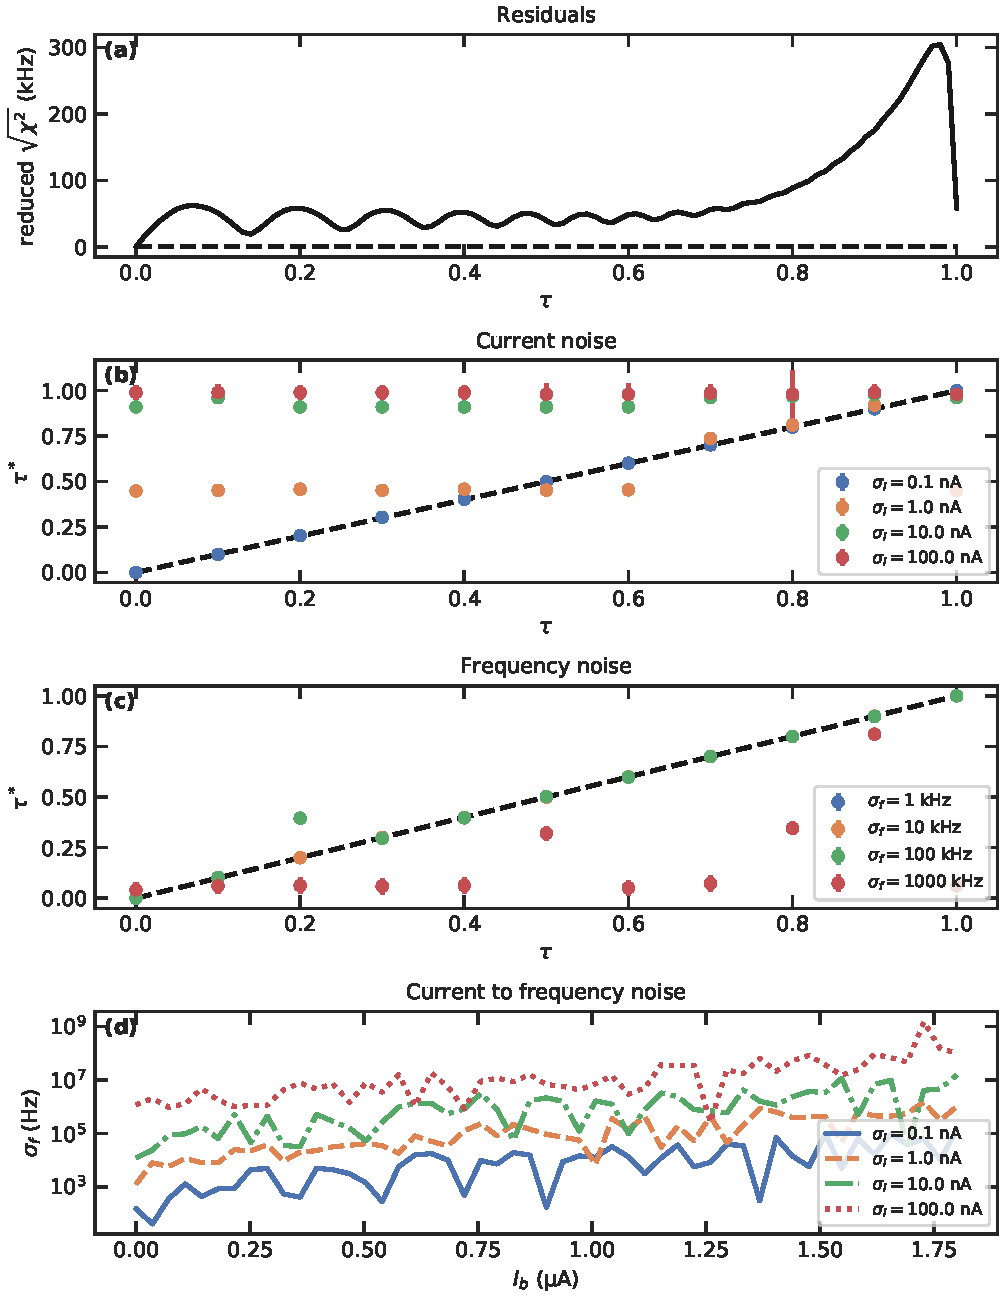
\includegraphics[width=\linewidth]{chapter-gJJ-CPR/figs/SMFigure-noise}
%	\caption{
%		\textbf{Influence of $\tau$ and noise on fit result.}
%		\textbf{(a)} Assuming a sinusoidal CPR for Eq.~\ref{eq:Pogorzalek} to fit data originating from a forward skewed CPR results in minimum fit residuals for $\tau=0$ (solid line).
%		%
%		Assuming the correct $\tau$ however results in minimum residuals (dashed line).
%		%
%		\textbf{(b-d)} Both current and frequency noise can significantly throw off the fitting algorithm by creating artificially global residual minima.
%		%
%		Plotted are calculations for $I_c=\SI{2}{\micro\ampere}$.
%		%
%		We estimate $\sigma_I<\SI{1}{\nano\ampere}$ in our setup.
%	}
%	\label{fig:SMres}
%\end{figure}

\clearpage
\references{dissertation}

